%documentclass sets the look of the whole document. you can try changing it around with the two commented out examples.

\documentclass{article}

%\documentclass{proc}
%\documentclass{beamer}

\usepackage{graphicx}
\title{Here is an example of how to use sub-files in LaTeX}

\author{XAM NOSLIW}

\begin{document}
\maketitle

%to include the table of contents just uncoment the line below. The newpage line would move the start of the document on the next page after the table of contents.
%\tableofcontents
%\newpage

\section{Shared Part}

This could be the Shared Part of the document. It is designed to be written by all members of the team.

Each member should ideally write their details in the table of contributors in the Shared Part of the document.



\subsection{Comments from the second student}
This is the first subsection. Do not forget to include the best parts about the module as well as what you did not like about Max Wilson during the term.

\subsection{Comments from the third student}
The best part of this term was the man-eating anteater attack. I did not like the fact Max used students as a human shield to protect himself during this trying time and I feel his feedback to the students that fought and died so valiantly could have been more constructive. However this was redeemed by the large donations he made in their names to anti-mad-scientist causes. 

\subsection{Comments from the forth student}
This is the first subsection. Do not forget to include the best parts about the module as well as what you did not like about Max Wilson during the term.

\subsection{Comments from the fifth student}
This is the first subsection. Do not forget to include the best parts about the module as well as what you did not like about Max Wilson during the term.

\subsection{Table of Contributors}


If you want to move a table around you will need to put some parameters in square brackets, if you want it exactly where it is positioned in the text editor just uncomment the [h] below, just after begin{table}

This is the table of contributors (Table~\ref{authors}):
\begin{table}%[h]
\centering
\caption{People in the Group}
\label{authors}
\begin{tabular}{|l|l|}
\hline
\textbf{Name} & \textbf{ID} \\
\hline
& \\
\hline
& \\
\hline
Alexi & psyajd \\
\hline
& \\
\hline
James Cordon & psyjmc \\
\hline
\end{tabular}
\end{table}
\newpage
\include{sections/FirstPart}
\newpage
\section{Second Member}
This is the section dedicated to one of the team members, and it should be written individually . It can include a range of things; first subsection is a space for you to point out the strengths and weaknesses of the module, including complaints about the module coordinator Max Wilson. The second section should have a selfie image with Max! The last part of it is the most important one. You will need to write a paragraph about what you have learned in this module. You can write it in \textbf{Bold} if you want or you can use other fonts. 

Please do not forget:
\begin{itemize}
	\item First paragraph should have your comments about the module
	\item Second one, a selfie img with Max
	\item Last one, what you learned in this module.
\end{itemize}

\subsection{Comments about the module}
I like working in a team and I like the lectures with the hand outs. 

\subsection{Selfie with Max}

To include an image, you will need to remove the comments from the code below, place an image in the main folder, and do not forget to put the name of the image instead of ImgName. 

%\begin{figure}[h]
%\caption{Selfie with Max}
%\centering
%\includegraphics[width=0.5\textwidth]{ImgName}
%\label{fig:selfie}
%\end{figure}

You can then use the label of the figure to reference it later with the command ${\backslash}ref.$ you can comment out the next line to see an example of how it works.

% My selfie with Max is in  Figure~\ref{fig:selfie}.

\subsection{What I have learned in this module}
I learnt how to do software engineering.


\newpage
\section{Third Member}
This is the section dedicated to one of the team members, and it should be written individually . It can include a range of things; first subsection is a space for you to point out the strengths and weaknesses of the module, including complaints about the module coordinator Max Wilson. The second section should have a selfie image with Max! The last part of it is the most important one. You will need to write a paragraph about what you have learned in this module. You can write it in \textbf{Bold} if you want or you can use other fonts. 

Please do not forget:
\begin{itemize}
	\item First paragraph should have your comments about the module
	\item Second one, a selfie img with Max
	\item Last one, what you learned in this module.
\end{itemize}

\subsection{Comments about the module}
This is the first subsection. Do not forget to include the best parts about the module as well as what you did not like about Max Wilson during the term.

\subsection{Selfie with Max}

\begin{figure}[h]
\caption{Selfie with Max}
\centering

\includegraphics[width=0.5\textwidth]{images/ACAMAX.jpg}
\label{fig:selfie}
\end{figure}

You can then use the label of the figure to reference it later with the command ${\backslash}ref$. you can comment out the next line to see an example of how it works.

% My selfie with Max is in  Figure~\ref{fig:selfie}.

\subsection{What I have learned in this module}
 Within this module I have learned the value of planning and strategy as well as strategies to implement to achieve goals such as requirement gathering or testing. 

\newpage
\section{Edward}
This is the section dedicated to Edward, and it was written individually . It includes a range of things; the first subsection is a space pointing out the strengths and weaknesses of the module, including complaints about the module coordinator Max Wilson. The second section is a selfie image with Max! The last part of it is the most important one. It is a paragraph about what Edward has learned in this module. 

Please do not forget:
\begin{itemize}
	\item First paragraph should have your comments about the module
	\item Second one, a selfie img with Max
	\item Last one, what you learned in this module.
\end{itemize}

\subsection{Comments about the module}
The best part of this module is working in a team as it allows me to blame others for my own mistakes.

\subsection{Selfie with Max}

To include an image, you will need to remove the comments from the code below, place an image in the main folder, and do not forget to put the name of the image instead of ImgName. 

\begin{figure}[h]
\caption{Selfie with Max}
\centering
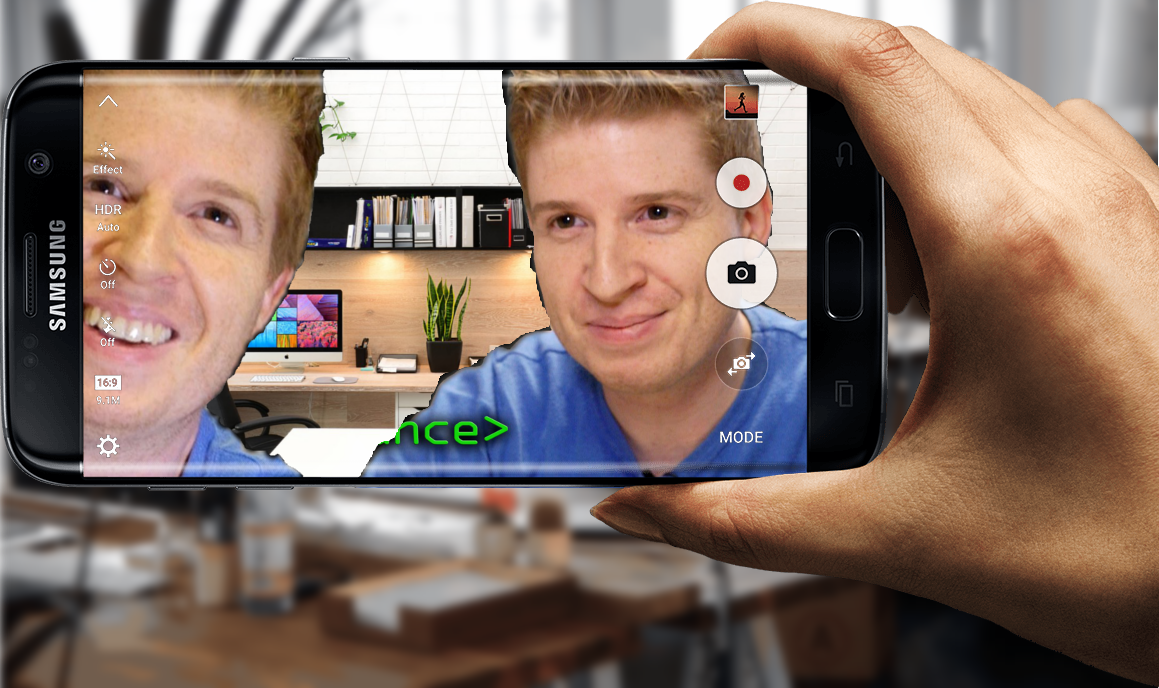
\includegraphics[width=0.5\textwidth]{images/mastapeece.png}
\label{fig:selfie}
\end{figure}

You can then use the label of the figure to reference it later with the command ${\backslash}ref$. you can comment out the next line to see an example of how it works.

% My selfie with Max is in  Figure~\ref{fig:selfie}.

\subsection{What I have learned in this module}
I have learnt an awful lot about the dos and don'ts of software engineering. 


\newpage
\section{James}
This is the section dedicated to one of the team members (namely, James), and it was written individually. It includes a range of things; first subsection is a space for him to point out the strengths and weaknesses of the module, including complaints about the module coordinator Max Wilson. The second section has a selfie image with Max! The last part of it is the most important one. He has written a paragraph about what he has learned in this module. Though he could have written it in \textbf{Bold} or other fonts, he chose not to, for this would have taken longer, and he thought that the default styling worked well enough. 

Please do not forget:
\begin{itemize}
	\item First paragraph should have your comments about the module
	\item Second one, a selfie img with Max
	\item Last one, what you learned in this module.
\end{itemize}

\subsection{Comments about the module}
All in all, I've found the Software Fundamentals module to be an interesting one. In the past, I've done both a GCSE and an A Level in Computer Science, and I've also written a variety of small programs and scripts for the past 7\(\frac{1}{2}\) years or so. Whilst doing those courses, there were components that required we show the software engineering process, and although it was to a lesser extent, it still involved the main ideas of requirements and specifications, a prototype, development and testing. Being able to see how to properly do these things (as opposed to writing the documents without really knowing why I needed to) is actually really useful, and I'm almost certain that it will come in useful in next year's group project!

\subsection{Selfie with Max}

\begin{figure}[h]
\caption{Selfie with Max}
\centering

\includegraphics[width=0.5\textwidth]{images/MJCMAX.jpg}
\label{fig:jamesselfie}
\end{figure}

You can then use the label of the figure to reference it later with the command ${\backslash}ref$. you can comment out the next line to see an example of how it works.

My selfie with Max is in  Figure~\ref{fig:jamesselfie}.

\subsection{What I have learned in this module}
In this module, I've learned the process of developing software, from specifications and requirements to ongoing maintenance. Hopefully this module will allow me to have a better time working in a team next year in the group project, as we will not try to start by immediately writing code.



\end{document}